\documentclass[a4paper]{article}
\usepackage[margin = 3cm]{geometry}
\usepackage[english]{babel}
\usepackage[utf8]{inputenc}
\usepackage{amsmath,amsthm}
\usepackage{amssymb}
\usepackage{graphicx, subfig}

\DeclareMathOperator{\N}{\mathcal{N}}

\title{Solving Fredholm integral equations of the first kind via Wasserstein gradient flow}
\author{Arnaud -> Adam, Francesca }
\date{ }

\begin{document}
\maketitle

\section{Fredholm integral equation of first kind}

We want to solve the integral equation
\[
\mu(y)=\int\rho\left(x\right)K(x,y)dx,
\]
where $\rho$ and $\mu$ are probability densities on $\mathbb{R}^{n}$ and $\mathbb{R}^{m}$ and $K$ a Markov transition density, i.e. $\mu=\rho K$ in operator notation. The solution to this problem is not unique and we propose to regularize the problem using an entropy constraint; i.e. for a given $\lambda>0$ we propose to minimize w.r.t. $\rho$
\[
E(\rho)=\text{{KL}}(\mu,\rho K)-\lambda\text{{Ent}}(\rho)
\]
where 
$\text{{KL}}(\mu,\rho K)$ is the Kullback-Leibler divergence between $\mu$ and $\rho K$ and $\text{{Ent}}(\rho)=-\int\rho\log\rho$ is the entropy of $\rho$.
This requires solving a minimization problem in the space of probability measures. We are going to follow a Wasserstein gradient flow approach.

\section{Gradient flow approach}
We first need to compute 
\[
\lim_{\epsilon\rightarrow0}\epsilon^{-1}\left(E(\rho+\epsilon\chi)-E(\rho)\right)=\int\frac{\delta E}{\delta\rho}\left(x\right)\chi\left(dx\right)
\]
where $\chi$ is any signed measure such that $\rho+\epsilon\chi$ is a probability measure. We have
\begin{align*}
E(\rho)= & \text{{KL}}(\mu,\rho K)-\lambda\text{{Ent}}(\rho)\\
=- & \int\mu\log\rho K+\lambda\int\rho\log\rho+\int\mu\log\mu.
\end{align*}
It follows directly that 
\[
\frac{\delta\text{{Ent}}\left(\rho\right)}{\delta\rho}=1+\log\rho.
\]
and 
\begin{align*}
\int\mu\log\left(\left(\rho+\epsilon\chi\right)K\right)-\int\mu\log\left(\rho K\right) & =\int\mu\left\{ \log\left(\rho K\right)+\log\left(1+\frac{\epsilon\chi K}{\rho K}\right)\right\} -\int\mu\log\left(\rho K\right)\\
 & =\int\mu\log\left(1+\frac{\epsilon\chi K}{\rho K}\right)\\
 & =\int\mu\left(\frac{\epsilon\chi K}{\rho K}+o\left(\frac{\epsilon\chi K}{\rho K}\right)\right)\\
 & =\epsilon\int\mu\frac{\chi K}{\rho K}+o\left(\epsilon\int\mu\frac{\chi K}{\rho K}\right).
\end{align*}
We have 
\[
\int\mu\frac{\chi K}{\rho K}=\int\int\mu\left(dy\right)\frac{K(x,y)}{\rho K(y)}d\chi\left(x\right)
\]
so 
\[
\frac{\delta \text{KL}}{\delta\rho}\left(x\right)=-\int\mu\left(dy\right)\frac{K(x,y)}{\rho K(y)}.
\]
Hence, it follows that 
\[
\frac{\delta E}{\delta\rho}\left(x\right)=-\int\mu\left(dy\right)\frac{K(x,y)}{\rho K(y)}+\lambda\left(1+\log\rho\left(x\right)\right).
\]
We can now compute the gradient of this functional derivative equation w.r.t. $x$
\[
\nabla\frac{\delta E}{\delta\rho}\left(x\right)=-\int\mu\left(dy\right)\frac{\nabla K(x,y)}{\rho K(y)}+\lambda\nabla\log\rho\left(x\right).
\]
We now consider the following PDE
\[
\partial_{t}\rho_{t}=\nabla\cdot\left(\rho_{t}\nabla\frac{\delta E}{\delta\rho_{t}}\right),
\]
where $\nabla\cdot f=\sum_{i}\partial_{i}f_{i}$ is the divergence operator.
The corresponding nonlinear ODE 
\begin{equation}
dX_{t}=-\nabla\frac{\delta E}{\delta\rho_{t}}\left(X_{t}\right)dt,\quad X_{0}\sim\rho_{0}\label{eq:nonlinearODE}
\end{equation}
is such that $Law(X_{t})=\rho_{t}$.
Then, by construction, one has
\[
\frac{dE\left(\rho_{t}\right)}{dt}=-\int\left\Vert \nabla\frac{\delta E}{\delta\rho_{t}}\left(x\right)\right\Vert ^{2}\rho_{t}\left(dx\right).
\]
The terminology nonlinear ODE is here used to indicate that the drift depends not only on $X_{t}$ but on its distribution too.

Practically, what we would like to do is to simulate $N$ particles $(X_{t}^{1},...,X_{t}^{N})$ such that, at initialization, we sample iid particles  $X_{0}^{i}\sim\rho_{0}$ and then implement numerically the $N$ nonlinear ODEs
\[
dX_{t}^{i}=\int\mu\left(dy\right)\frac{\nabla K(X_{t}^{i},y)}{\rho_{t}^{N}K(y)}dt-\lambda\nabla\log\left(\rho_{t}^{N}*H_{\epsilon}\left(X_{t}^{i}\right)\right)dt,\quad\rho_{t}^{N}=\frac{1}{N}\sum_{i=1}^{N}\delta_{X_{t}^{i}}.
\]

Approximating the first term on the r.h.s. is fine as practically $\mu\left(dy\right)$ is a discrete measure but approximating $\nabla\log\rho_{t}\left(x\right)$ from the empirical measure $\rho_{t}^{N}$ is difficult and would require say convolution by some kernel $H_{\epsilon}$.
This is ugly and would be most likely highly inefficient.
In the next section, we show how to address this issue.

\section{Nonlinear SDE approach and numerical implementation}

Let us rewrite the PDE 
\begin{align*}{1}
\partial_{t}\rho_{t}= & \nabla\cdot\left(\rho_{t}\nabla\frac{\delta E}{\delta\rho_{t}}\right)\\
= & -\nabla\cdot\left(\rho_{t}\int\mu\left(dy\right)\frac{\nabla K(x,y)}{\rho_{t}K(y)}\right)+\lambda\nabla\cdot\left(\rho_{t}\nabla\log\rho_{t}\right).
\end{align*}
However, we have
\[
\nabla\cdot\left(\rho_{t}\nabla\log\rho_{t}\right)=\nabla\cdot\nabla\rho_{t}=\triangle\rho_{t},
\]
where $\triangle f=\sum_{i}\partial_{i}^{2}f_{i}$ is the Laplacian.
So we can consider the following non-linear SDE (McKean-Vlasov) 
\begin{equation}
dX_{t}=\int\mu\left(dy\right)\frac{\nabla K(X_{t},y)}{\rho_{t}K(y)}dt+\sqrt{2\lambda}dW_{t},\quad X_{0}\sim\rho_{0},\label{eq:nonlinearSDE}
\end{equation}
where $W_{t}$ is a standard $n-$dimensional Brownian motion.
The SDE \eqref{eq:nonlinearSDE} has the same marginal distributions as the nonlinear ODE \eqref{eq:nonlinearODE}.
So to solve the minimization problem of interest, we will simulate in practice $N$ particles $(X_{t}^{1},...,X_{t}^{N})$ such that, at initialization, we sample iid particles $X_{0}^{i}\sim\rho_{0}$ and then they evolve according to the non-linear (McKean-Vlasov) SDE
\[
dX_{t}^{i}=\int\mu\left(dy\right)\frac{\nabla K(X_{t},y)}{\rho_{t}^{N}K(y)}dt+\sqrt{2\lambda}dW_{t}^{i},\quad\rho_{t}^{N}=\frac{1}{N}\sum_{i=1}^{N}\delta_{X_{t}^{i}}.
\]

We will also need to further discretize in time these SDEs obviously.

\section{Toy Example}

We consider the toy Fredholm integral equation
\begin{equation*}
\N(y; m, \sigma_{\rho}^2 + \sigma_K^2) = \int \N(x; m, \sigma_{\rho}^2)\N(y; x, \sigma_K^2)\ dx,\qquad y\in\mathbb{R}.
\end{equation*}
Figure \ref{fig:at} shows the reconstruction of $\N(x; m, \sigma_{\rho}^2)$ with $m=0.5$, $\sigma_{\rho}^2 = 0.043^2$, $\sigma_K^2 = 0.045^2$.
We set $N=10^{4}$, $\lambda = 10$, $dt = 10^{-3}$. The initial distribution $\rho_0$ is uniform on $[0, 1]$.

\begin{figure}
\centering
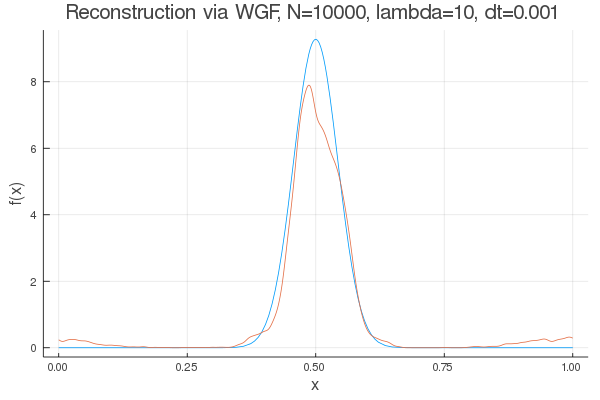
\includegraphics[width = 0.8\textwidth]{analitically_tractable}
\caption{ }
\label{fig:at}
\end{figure}
\end{document}